%------------------------------------------------------------------------------%
%                                   planning                                   %
%------------------------------------------------------------------------------%

\clearpage{}
\section{Planning}

In this section, we will compare the expected planning with the real one by
commenting two Gantt charts.\\

The figure \ref{fig:expectedgantt} shows the expected Gantt chart for this
project. On this chart, we can see that the first month was dedicated to the
learning of \gls{hh}. The second task was the implementation of the Cholesky
decomposition (the chart has been made when this task has started; this
corresponds to our first meeting at the NIST). Then, the other tasks correspond
to the port of \gls{fds} to \gls{hh}. Originally it was planned to work
exclusively on \gls{fds} and to complete the project before the end of the
internship. Unfortunately, as we saw earlier that we eventually decided to adopt
another method in the middle of the project.

% [Expected gantt chart] {{{
\begin{figure}[h!]
  \begin{center}
    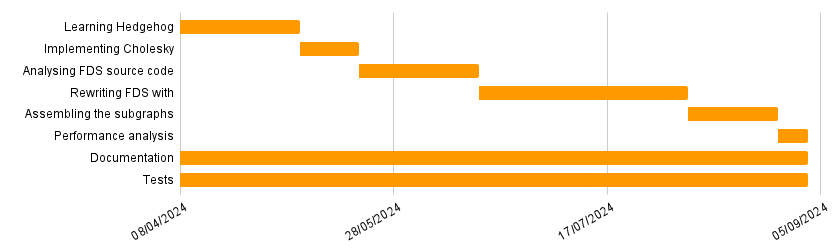
\includegraphics[scale=0.5]{img/expected-gantt-chart.png}
    \caption{Expected Gantt chart}
    \label{fig:expectedgantt}
  \end{center}
\end{figure}
%}}}

On the real Gantt chart, visible on the figure \ref{fig:realgantt}, we can see
that the tasks of learning \gls{hh} and implementing the Cholesky decomposition
are still there. However, there are some new tasks on this second chart.
Firstly, there is the work on the 3D loops program. When we started the project,
we did not have the knowledge of this test program. We decided to work on it
after the \gls{fds}'s developers presented it to us. Then, as we have seen in
the report, optimizing \gls{fds} by hand was too complicated, so we decided to
implement a tool that could automate a part of the task. Finally, since it has
been proposed to use the serialization library during the internship, this task
only appears in the real Gantt chart.

% [Real gantt chart] {{{
\begin{figure}[h!]
  \begin{center}
    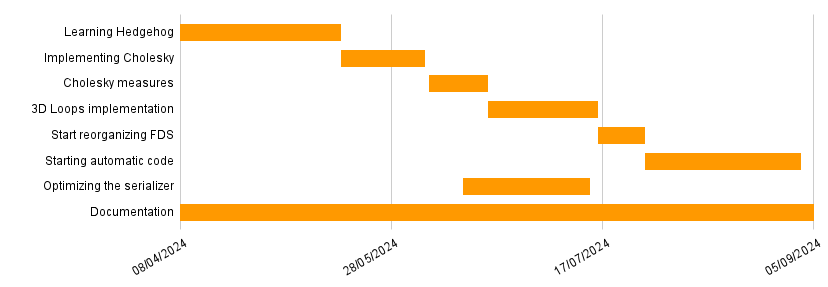
\includegraphics[scale=0.5]{img/real-gantt-chart.png}
    \caption{Real Gantt chart}
    \label{fig:realgantt}
  \end{center}
\end{figure}
%}}}

Those diagrams are very different for two reasons. Firstly, it is difficult to
evaluate the work on an unknown code base, such as the \gls{fds}'s one.
Secondly, the usage of the serialization library and the implementation of the
refactoring tool were propositions that have been made during the project, with
some knowledge and observations that we did not have originally.
